\section{Results}
\subsection{Data Pre-processing}
This section would cover the actual experimentation done in this research. The pre-processing of data, the results for different range of prediction, and the findings from the results will be written accordingly. In this paper, two kinds of predictions were done; Univariate Prediction, and Multivariate Prediction. Univariate Prediction is a prediction procedure which uses only the past data of the objective value for predictions. On the other hand, Multivariate Prediction refers to the prediction procedure using multiple features to predict the objective value. We would like to focus on the accuracy of our models when handling multiple features into the data as well as the efficacy of deep learning models compared to conventional linear methods. 

\subsubsection{Stationarity}
As mentioned in section 2.2.2, stationary diagnostic is imperative to avoid spurious prediction results. Therefore we use the Augmented Dickey-Fuller (ADF) test to determine stationarity in our dataset. This paper would conduct a \textit{Student-t Hypothesis test} shown in (\ref{eq:ADF_hypothesis}) using the test statistic shown in (\ref{eq:ADFt}) for all data features. We set multiple significance level ($10\%, 5\%, 1\%$) to see how the extent of stationarity the data features are able to achieve. Below would be a table showing the result of ADF test before pre-processing the data.

\begin{table}[ht]
\centering
\caption{\label{tab:ADF1st}ADF 1st Test}
\begin{tabular}{ |p{4cm}||p{1.7cm}|p{1.7cm}|p{1.7cm}|p{1.7cm}|p{2.3cm}| }
 \hline
 \multicolumn{6}{|c|}{ADF Test results by Features} \\
 \hline
 Data Feature & Test Statistic & 1\% Significance & 5\% Significance & 10\% Significance & Pass/Reject\\
 \hline
\textit{Hospitalized} & -3.2875 & -3.4413 & -2.8664 & -2.5693 & Reject at 1\% \\
\textit{Light-Mid\_Symptoms} & -3.2277 & -3.4413 & -2.8664 & -2.5693 & Reject at 1\% \\
\textit{Severe\_Symptoms} & -3.1195 & -3.4415 & -2.8665 & -2.5694 & Reject at 1\% \\
\textbf{Dead} & -1.9363 & -3.4414 & -2.8664 & -2.5694 & Reject at 10\% \\
Discharged & -3.6668 & -3.4414 & -2.8664 & -2.5694 & Pass \\
PCR\_Positive & -3.9643 & -3.4415 & -2.8665 & -2.5694 & Pass \\
\textbf{PCR\_Negative} & -2.1540 & -3.4415 & -2.8665 & -2.5694 & Reject at 10\% \\
\textbf{Tested\_MA(7days)} & -2.3580 & -3.4415 & -2.8664 & -2.5694 & Reject at 10\% \\
Positive\_Rate & -3.6516 & -3.4414 & -2.8664 & -2.5694 & Pass \\
ComparisonPreDay & -6.7442 & -3.4414 & -2.8664 & -2.5694 & Pass \\
ComparisonPreDeclare & -3.9288 & -3.4414 & -2.8664 & -2.5694 & Pass \\
ComparisonPreSpread & -4.1440 & -3.4414 & -2.8664 & -2.5694 & Pass \\
 \hline
\end{tabular}
\end{table}

Looking at the Test Statistic column of Table \ref{tab:ADF1st}, we see the test statistic for the corresponding features and the critical values for all the significance level that we have set. The rejected features are emphasised within the table and we can see features, \textbf{Dead}, \textbf{PCR\_Negative} and \textbf{Tested\_MA(7days)} demonstrate high non-stationarity being rejected at the siginificance level of 10\%, and features, \textit{Hospitalized}, \textit{Light-Mid\_Symptoms}, \textit{Severe\_Symptoms} demonstrates some non-stationarity which is rejected at the significance level of 1\%. These features all requires data pre-processing of taking the first difference which is shown in equation (\ref{eq:First_Difference}).

After we modify the dataset by taking the first difference, we determine once again for stationarity using ADF test. Below would be the result of the second ADF test. 
\begin{table}[ht]
\centering
\caption{\label{tab:ADF2nd}ADF Test after Taking the First Difference for Rejected Features}
\begin{tabular}{ |p{4cm}||p{1.7cm}|p{1.7cm}|p{1.7cm}|p{1.7cm}|p{2.5cm}| }
 \hline
 \multicolumn{6}{|c|}{ADF Test results by Features} \\
 \hline
 Data Feature & Test Statistic & 1\% Significance & 5\% Significance & 10\% Significance & Pass/Reject\\
 \hline
Hospitalized & -5.8545 & -3.4414 & -2.8664 & -2.5694 & Pass \\
Light-Mid\_Symptoms & -5.9519 & -3.4414 & -2.8664 & -2.5694 & Pass \\
Severe\_Symptoms & -4.3166 & -3.4415 & -2.8665 & -2.5694 & Pass \\
Dead & -8.2268 & -3.4414 & -2.8664 & -2.5694 & Pass \\
PCR\_Negative & -7.6164 & -3.4415 & -2.8665 & -2.5694 & Pass \\
Tested\_MA(7days) & -4.4329 & -3.4415 & -2.8664 & -2.5694 & Pass \\
 \hline
\end{tabular}
\end{table}

As demonstrated in Table \ref{tab:ADF2nd}, we can see that all features of data passes the ADF test at all significance level. Therefore, we can confirm that we have a dataset which all features are stationary and precludes the problematic statistical features which affects the prediction results. 

\subsubsection{Multicollinearity}
Multicollinearity is also a statistical property in time series data, which should be avoided in predictive models. As demonstrated in Section 2.2.4, multicollinerarity is a linear relationship within data features in the independent variable which undermines the statistical significance of the independent variable by making the partial regression coefficient highly volatile. We check for multicollinearity using Variance Inflation Factor (VIF) which is computed by equation (\ref{eq:VIF}). Table \ref{tab:VIF1st} is the table which shows the value of VIF before any pre-processing procedures.  

\begin{table}[h]
\centering
\caption{\label{tab:VIF1st}VIF values determining Multicollinearity}
\begin{tabular}{ |p{5cm}||p{2cm}| }
 \hline
    Data Feature &  VIF\\
 \hline
\textbf{Hospitalized} & \textbf{inf} \\
\textbf{Light-Mid\_Symptoms} & \textbf{inf} \\
\textbf{Severe\_Symptoms} & \textbf{inf} \\
Dead & 1.0716 \\
Discharged & 3.3515 \\
PCR\_Positive & 4.0029 \\
PCR\_Negative & 1.8314 \\
Tested\_MA(7days) & 1.2787 \\
ComparisonPreDay & 1.0452 \\
\textbf{ComparisonPreDeclare} & \textbf{55.2256} \\
\textbf{ComparisonPreSpread} & \textbf{52.9435} \\
 \hline
\end{tabular}
\end{table}

The threshold of VIF whether the data features suggest multicollinearity is $VIF\geq 10$. Looking at Table \ref{tab:VIF1st} we can see several features which induces multicollinearity. We first see the first three columns; \textbf{Hospitalized}, \textbf{Light-Mid\_Symptoms}, and \textbf{Severe\_Symptoms} having \textbf{inf} value for its VIF. Looking at Figure \ref{fig:multicollinearity}, the features in this example which are \textbf{Hospitalized} and  \textbf{Light-Mid\_Symptoms} show high correlation and can estimate that these data demonstrates a linear relationship. Therefore, we exclude the \textbf{Hospitalized} column to avoid multicollinearity. The other modification we can suggest is to exclude one of the human foot traffic data, which have an identical data generation process of comparing the traffic data with the past traffic data. Therefore, this paper will exclude \textbf{ComparisonPreDeclare} which presents a higher value in $VIF$ than other foot traffic data. Through the modifications of dropping two features within our dataset we get the set of $VIF$ shown in Table \ref{tab:VIF2nd}.

\begin{table}[h]
\centering
\caption{\label{tab:VIF2nd}VIF values After Removing Columns of Similar Data Characteristic}
\begin{tabular}{ |p{5cm}||p{2cm}| }
 \hline
    Data Feature &  \textit{VIF}\\
 \hline
Light-Mid\_Symptoms & 1.1573 \\
Severe\_Symptoms & 1.3379 \\
Dead & 1.0643 \\
Discharged & 3.3244 \\
PCR\_Positive & 3.9300 \\
PCR\_Negative & 1.1438 \\
Tested\_MA(7days) & 1.2724 \\
ComparisonPreDay & 1.0343 \\
ComparisonPreSpread & 1.0407 \\
 \hline
\end{tabular}
\end{table}

From the table above, we can see that all values of VIF have dropped to an insignificant level of $VIF\leq10$.  Therefore, by the modifications of dropping identical data features, we can confirm that all independent variables in the dataset does not present multicollinearity and can be used simultaneously in our prediction models. There are other ways to remedy multicollinearity such as combining two similar datasets into a single feature. However, the combining process has to be well planned with extensive knowledge about the data itself and the interdependencies between the combining features. Hence, this paper would take the simple step of excluding features to alleviate multicollinearity.

\subsection{Specification of Results}
Using the pre-processed dataset, we constructed several models to predict the \textbf{Positive Rate} observed in Tokyo. Below would be a description of the used dataset in this subsection. 

\begin{itemize}
    \item Objective Value: Positive\_Rate
    \item Features: Light-Mid\_Symptoms, Severe\_Symptoms, Dead,
       Discharged, PCR\_Positive, PCR\_Negative, Tested\_MA(7days),
       ComparisonPreDay, ComparisonPreSpread (9 Features)
    \item Total Data Date Range: 2020/05/02-2021/12/30 (length=608)
    \item Train Data Date Range for 40 days prediction: 2020/05/02-2021/11/20 (length=568)
    \item Test Data Date Range for 40 days prediction: 2021/11/21-2021/12/30 (length=40)
    \item Train Data Date Range for 80 days prediction: 2020/05/02-2021/10/11 (length=528)
    \item Test Data Date Range for 80 days prediction: 2021/10/12-2021/12/30 (length=80)
    \item Train Data Date Range for 20 days prediction: 2020/05/02-2021/12/10 (length=588)
    \item Test Data Date Range for 20 days prediction: 2021/12/11-2021/12/30 (length=20)
    \item Validation split: 10\% of training data

\end{itemize}

This paper would evaluate the model based on the computation of the loss function, Root Mean Squared Error (RMSE) which is defined as:
\begin{equation}\label{eq:RMSE}
    \mathrm{RMSE}=\sqrt{\frac{1}{n} \sum_{i=1}^{n}\left(y_{i}-\hat{y}_{i}\right)^{2}}
\end{equation}
where $y_{i}$ and $\hat{y}_{i}$ each denoting the actual value and prediction value respectively. The prediction results from models would be quantitatively evaluated based on the RMSE value of prediction results and qualitatively evaluated using the line plots of the predicted values. Also, in the line plot used below, the test data would be labeled in the color blue, and the predicted value in orange. 

For the neural network models, this paper constructed a 5 layer network with unit size of 128, 256, 128, 64 and an output layer. The activation function used in between the layers is LeakyReLU \citep{LeakyReLU} with $alpha=0.1818$ ($a=5.5$ in \ref{eq:LeakyReLU}) and a dropout layer of 40\% is added in between all hidden layers. The optimizer used in the models were Adam optimizer and each of the models were trained for 500 epochs with a batch size of 32. The input size which stores the amount of past values to be used for prediction is altered within the range of predictions; for 40days prediction, the input size is 14days, for 20days prediction, the input size is 7days, and for 80 days prediction, the input size is 21days. Each taking their respective input size, the neural network will use the input size data to predict one future value. 

\subsection{40 Days Prediction}
40 day prediction is done for standard prediction. By evaluating the performances of this prediction, we are able to understand the models capability of making a general prediction.

\subsubsection{Univariate Model (40 Days)}
The ARMA model used in this section was ARMA(2,2) which had the lowest AIC \citep{AIC} within the tested range of lags ranging from 0 to 7. 

\begin{table}[h]
\caption{Univariate Prediction Performance of Each Model (Best To Worst) - 40 Days Prediction}
    \label{tab:40Uni}
    \centering
    \begin{tabular}{ |p{3cm}||p{3cm}| }
        \hline
         Model &  RMSE\\
        \hline
        \textbf{GRU}  & \textbf{0.000849}\\
        ARMA(2,2) & 0.002174\\
        LSTM  & 0.004307\\
    \hline
    \end{tabular}
\end{table}

Table \ref{tab:40Uni} shows the result of the predictions. GRU was able to predict with a high accuracy with a RMSE value smaller than the ARMA model by 256\%. On the other hand, the LSTM mdoel did not perform well in its predictions with RMSE value bigger than ARMA by 198\%. 

\begin{figure}[!ht]
    \centering
    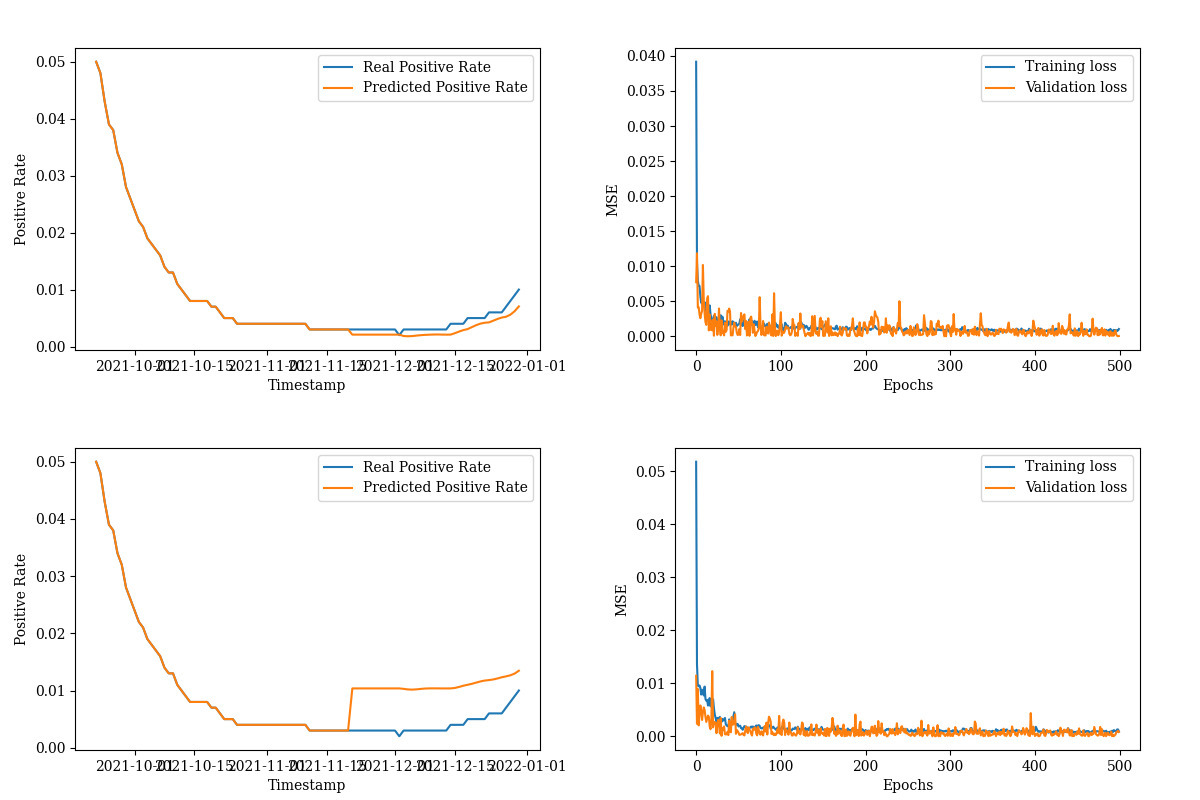
\includegraphics[width=16cm]{images/DeepLearning_Uni_40days.png}
    \captionof{figure}{The line graph of produced prediction results and process of accuracy performance of univariate prediction of 40 days. Looking at the prediction results of GRU (top-left), we could see that the neural network is able to predict the objective value by a high accuracy. On the other hand, the prediction results of LSTM (bottom-left) shows a spike in its first prediction, but able to track the upward trend in the end. The accuracy performance of both GRU (top-right) and LSTM (bottom-right) shows that the validation loss is decreasing but oscillates in small margins. Furthermore, we can see that the variance of oscillation decreases as the epochs increase.}
    \label{fig:DL_Uni_40}
\end{figure}

\begin{figure}[!ht]
    \centering
    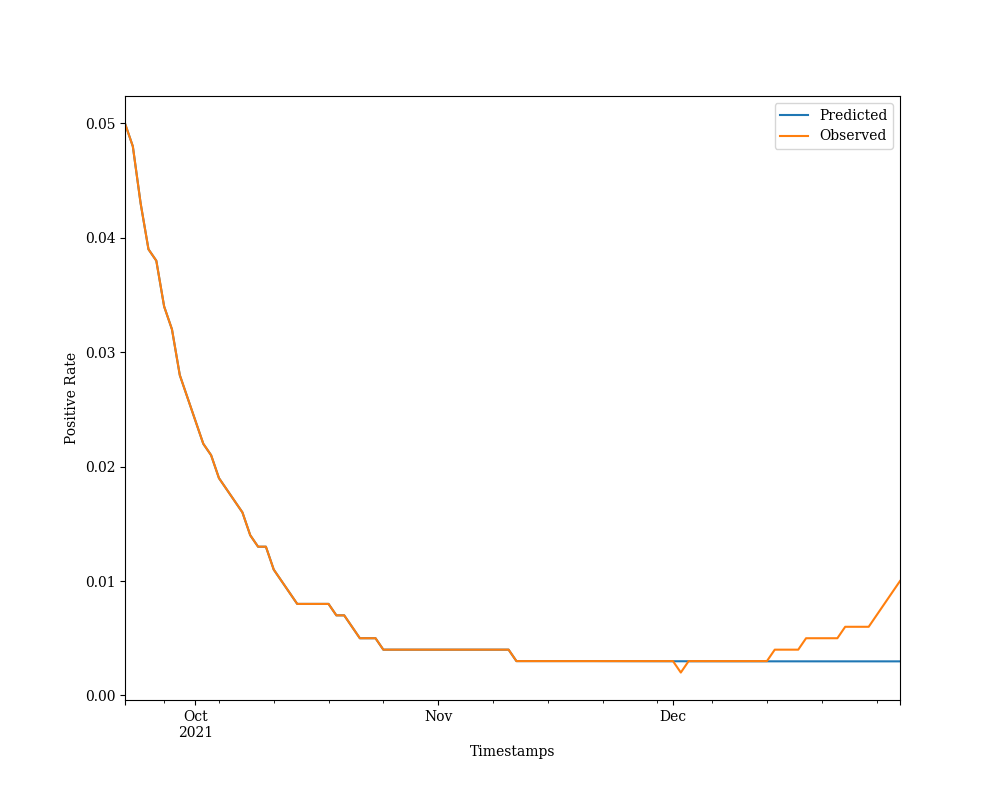
\includegraphics[width=8cm]{images/ARIMA(2,1,2)_40Days.png}
    \captionof{figure}{The line graph of produced 40 days prediction result from the ARMA(2,2) model. We could see that the prediction is static and is not changing its value at the end.}
    \label{fig:ARMA_Uni_40_line}
\end{figure}

Figures \ref{fig:DL_Uni_40}, \ref{fig:ARMA_Uni_40_line} shows the line graph of the prediction and the real data. As indicated from the RMSE, the GRU fitted very well with the actual data. Looking at the ARMA model, we could see that the prediction is static and does not accurately illustrate the slight rise of number in the end. LSTM had a spike in the first prediction but after the spike, the shape of the line plot seems to reflect the actual values. Overall, GRU model was able to accurately predict the value in a big margin compared with other models. 



\subsubsection{Multivariate Model (40 Days)}
For the conventional model VARMA(2,3) is used. Due to the long computational time the fitting of Auto Regressive model consumes, features used in VARMA needed to be truncated. Therefore in this model, the features Positive\_Rate, Discharged, PCR\_Positive, and ComparisonPreSpread was used for this model since each of the features showed high correlation between the objective variable. The neural network model each used all the features in the dataset for the predictions. 
\begin{table}[h]
\caption{Multivaraite Prediction Performance of Each Model (Best To Worst) - 40 Days Prediction}
    \label{tab:40Mult}
    \centering
    \begin{tabular}{ |p{3cm}||p{3cm}| }
        \hline
         Model &  RMSE\\
        \hline
        \textbf{GRU}  & \textbf{0.015485}\\
        VARMA(2,3) & 0.021116\\
        LSTM  & 0.030772\\
    \hline
    \end{tabular}
\end{table}

\begin{figure}[!ht]
    \centering
    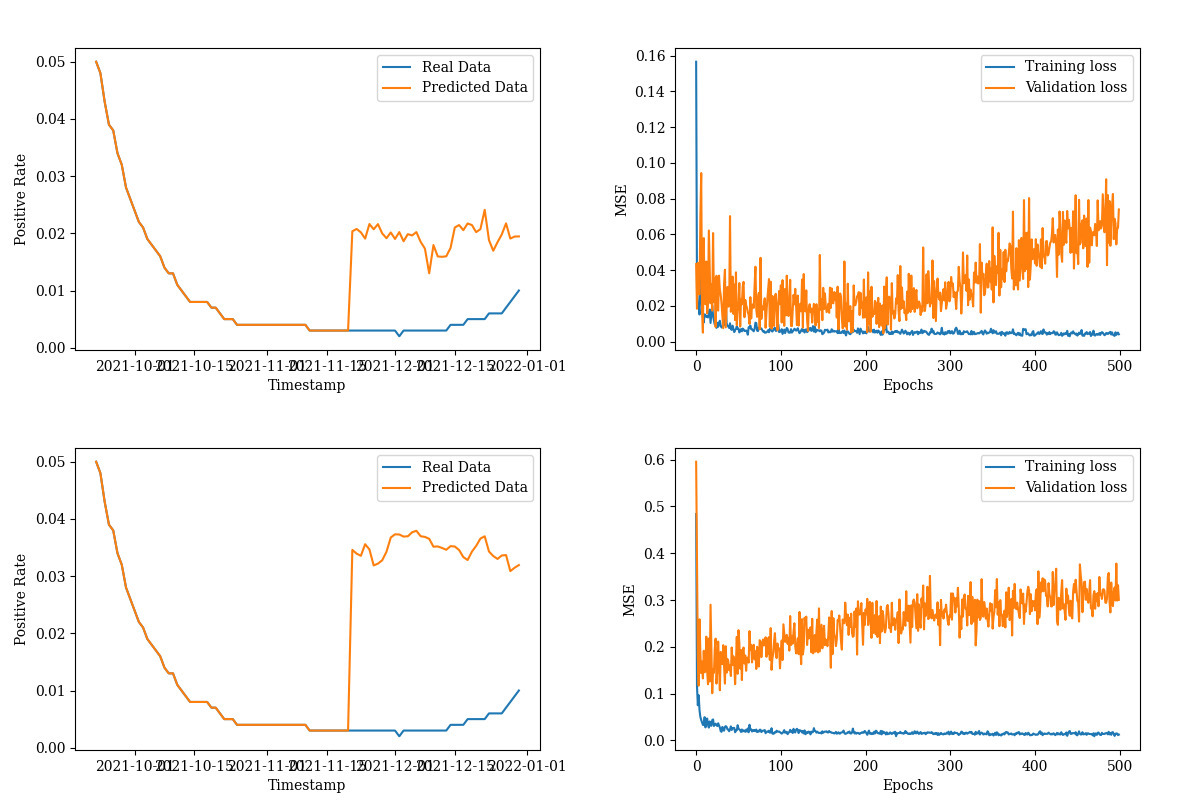
\includegraphics[width=16cm]{images/DeepLearning_Mult_40Days.png}
    \captionof{figure}{The line graph of produced prediction results and process of accuracy performance of multivariate prediction of 40 days. Looking at the prediction results of GRU (top-left) and LSTM (bottom-left) we could see that the model was not able to predict the objective value with high accuracy. They both have a very big spike in its prediction and has a fluctuation which is not observed in real data. The accuracy performance of both GRU (top-right) and LSTM (bottom-right) shows that despite the training loss is able to decrease its value the validation loss is increasing as the epochs increase. This indicates a characteristic of over-fitting and is not versatile in its predictions.}
    \label{fig:DL_Mult_40}
\end{figure}

\begin{figure}[!ht]
    \centering
    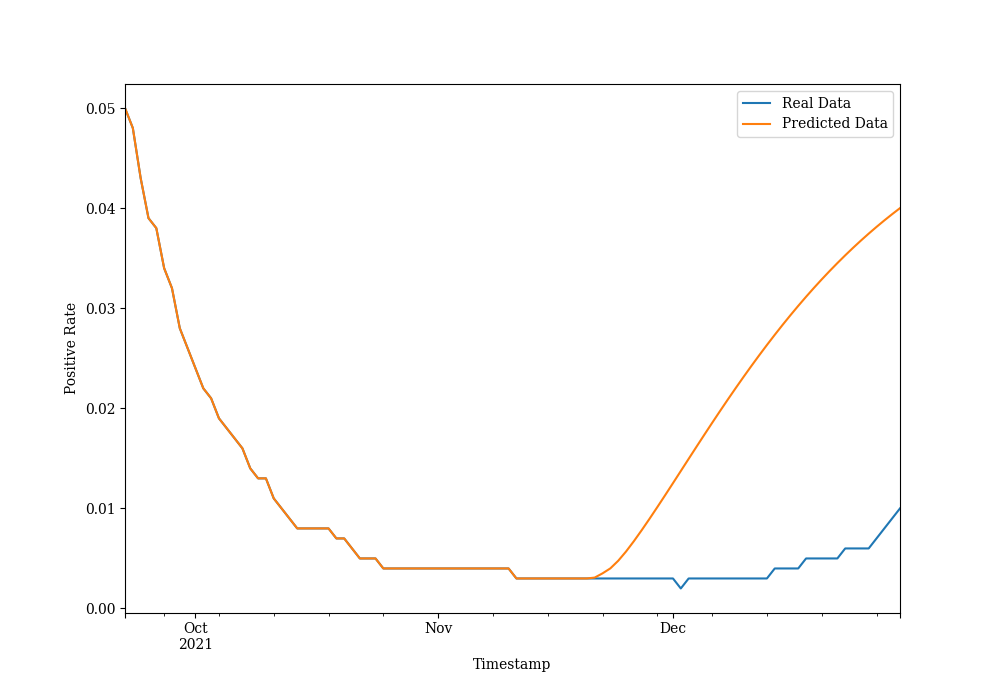
\includegraphics[width=8cm]{images/VARMA(2,3)_40Days.png}
    \captionof{figure}{The line graph of produced 40 days prediction results from the VARMA(2,3) model. We could see that the model is able to capture the upward trend in the objective value but the margin between the real data is large. We could also see that the predicted value is smoother compared to the neural network prediction results.}
    \label{fig:VARMA_Mult_40_line}
\end{figure}

Table \ref{tab:40Mult} shows the value of RMSE for the predicted value and the actual value. Looking at the RMSE the multivariate prediction was unsuccessful in making an accurate prediction when compared with the prediction results of the univariate predictions. Figure \ref{fig:DL_Mult_40} and  \ref{fig:VARMA_Mult_40_line} shows the prediction results. We can see that none of the models showed a very big spike in its prediction values. Judging from the Accuracy Performance in Figure \ref{fig:DL_Mult_40} the neural network fitted excessively with the training data and did not perform well in the validation dataset. Therefore showing signs of overfitting in our model. Overall, compared to the results of univariate predictions, we can conclude that the increase in features used in the model have worsened the prediction results. 

\subsection{20 Days Prediction}
20 day prediction is done to check the performances for the short term predictions. The performances in this model determines the model's capability of interpreting long sequential patterns in the training data and extract the slight upward trend existing in the end of the data. 
\subsubsection{Univariate Model (20 Days)}
For the conventional model of ARMA for univariate prediction of 20days, ARMA(2,2) model will be used. 
\begin{table}[h]
\caption{Univariate Prediction Performance of Each Model (Best To Worst) - 20 Days Prediction}
    \label{tab:20Uni}
    \centering
    \begin{tabular}{ |p{3cm}||p{3cm}| }
        \hline
         Model &  RMSE\\
        \hline
        \textbf{LSTM}  & \textbf{0.002800}\\
        ARMA(2,2) & 0.003043\\
        GRU  & 0.003290\\
    \hline
    \end{tabular}
\end{table}

Table \ref{tab:20Uni} shows the performance of the models. For the prediction of 20 days, LSTM performed better than the ARMA model and also the GRU model. However, judging from the small difference in RMSE, we cannot indicate a significant difference in its performances. 

\begin{figure}[!ht]
    \centering
    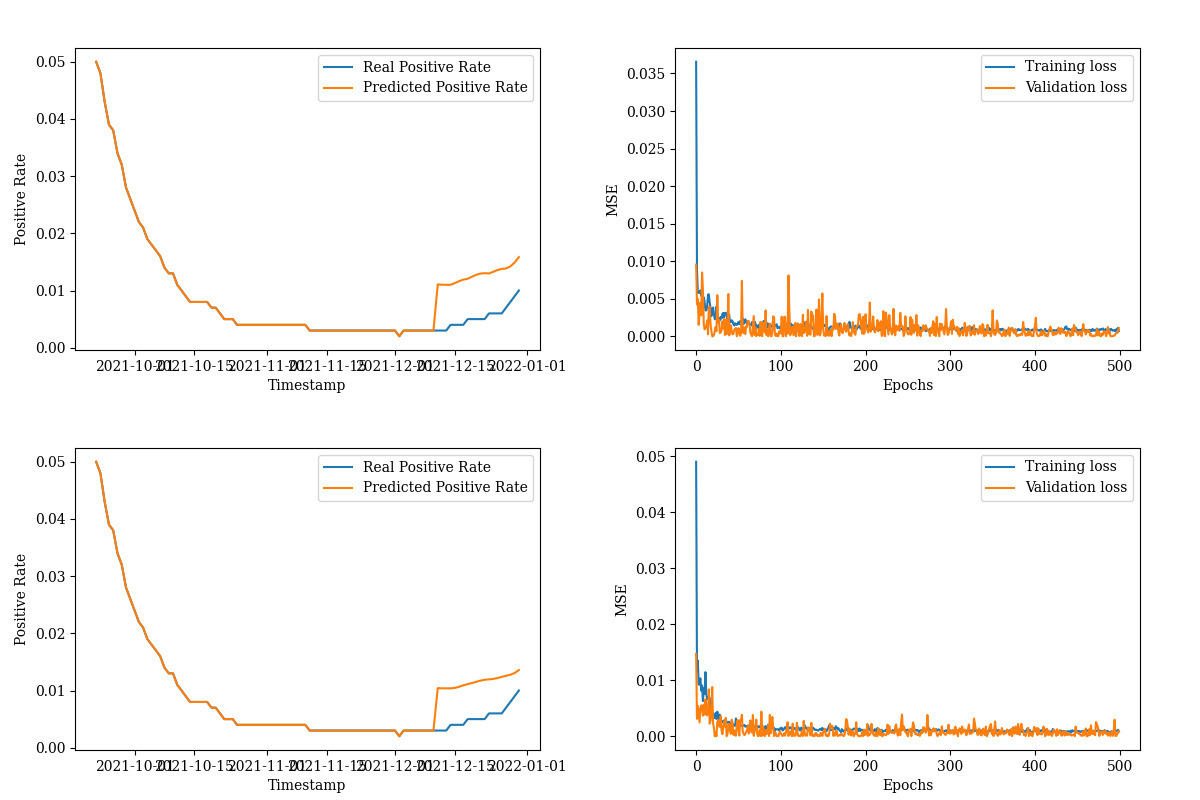
\includegraphics[width=16cm]{images/DeepLearning_Uni_20Days.jpg}
    \captionof{figure}{The line graph of produced prediction results and process of accuracy performance of the univariate prediction of 20 days. Looking at the prediction results of GRU (top-left) and LSTM (bottom-left) both shows a spike in its first prediction, but able to track the upward trend towards the end. The accuracy performance of both GRU (top-right) and LSTM (bottom-right) shows that the validation loss is decreasing with its training loss. In comparison however, it can be seen that the training accuracy is decreasing more in the LSTM model.}
    \label{fig:DL_Uni_20}
\end{figure}

\begin{figure}[!ht]
    \centering
    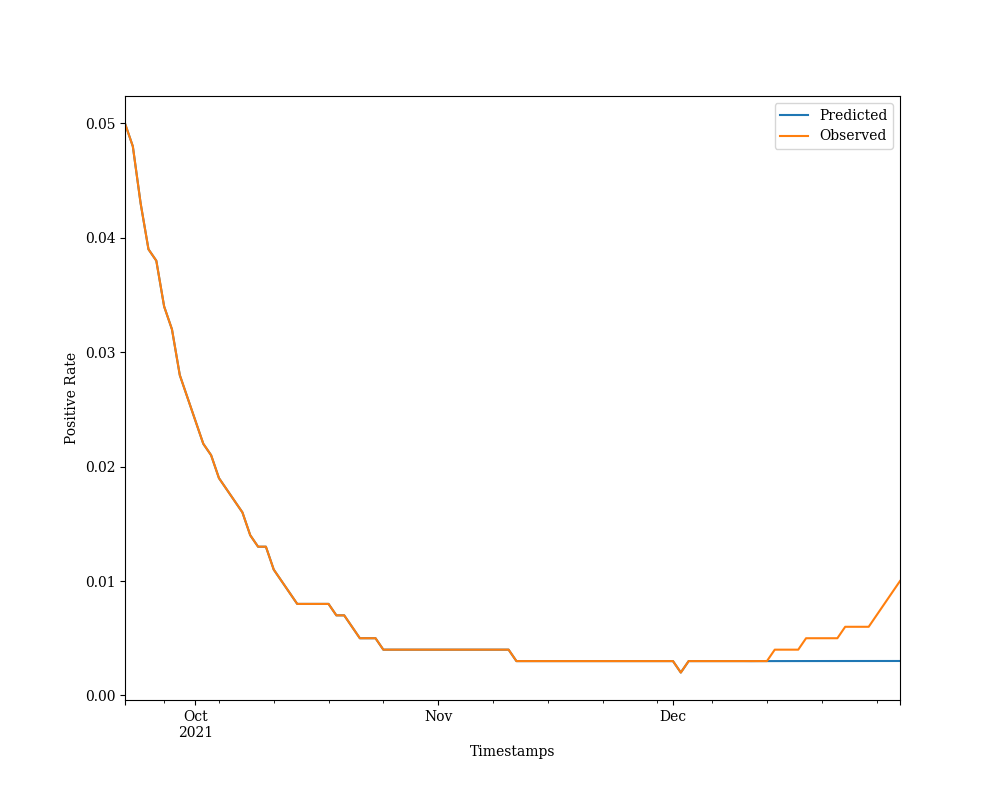
\includegraphics[width=8cm]{images/ARIMA(2,1,2)_20Days.png}
    \captionof{figure}{The line graph of produced 20 days prediction results of ARMA(2,2) model. We could see that the prediction is static and is not changing its value.}
    \label{fig:ARMA_Uni_20_line}
\end{figure}

Figure \ref{fig:DL_Uni_20}, \ref{fig:ARMA_Uni_20_line} shows the prediction values of the corresponding models. We can see that the neural network both present a spike for the first prediction value but captures the overall trend of the change of values. We can also see that the neural network model captures the upward trend in the end while the ARMA model does not present any change in its prediction value and is static. Overall, neither of the model does not demonstrate a good fit for a prediction model. 

\subsubsection{Multivariate Model (20 Days)}
Same as the VARMA model for 40days prediction, features had to be reduced to conduct the prediction. Therefore, features Positive\_Rate, Discharged, PCR\_Positive, and ComparisonPreSpread were used and the appropriate lag was estimated at VARMA(7,2). 
\begin{table}[h]
\caption{Multivariate Prediction Performance of Each Model (Best To Worst) - 20 Days Prediction}
    \label{tab:20Mult}
    \centering
    \begin{tabular}{ |p{3cm}||p{3cm}| }
        \hline
         Model &  RMSE\\
        \hline
        VARMA(7,2) & 0.005607\\
        LSTM  & 0.007889\\
        GRU  & 0.008213\\
    \hline
    \end{tabular}
\end{table}

\begin{figure}[!ht]
    \centering
    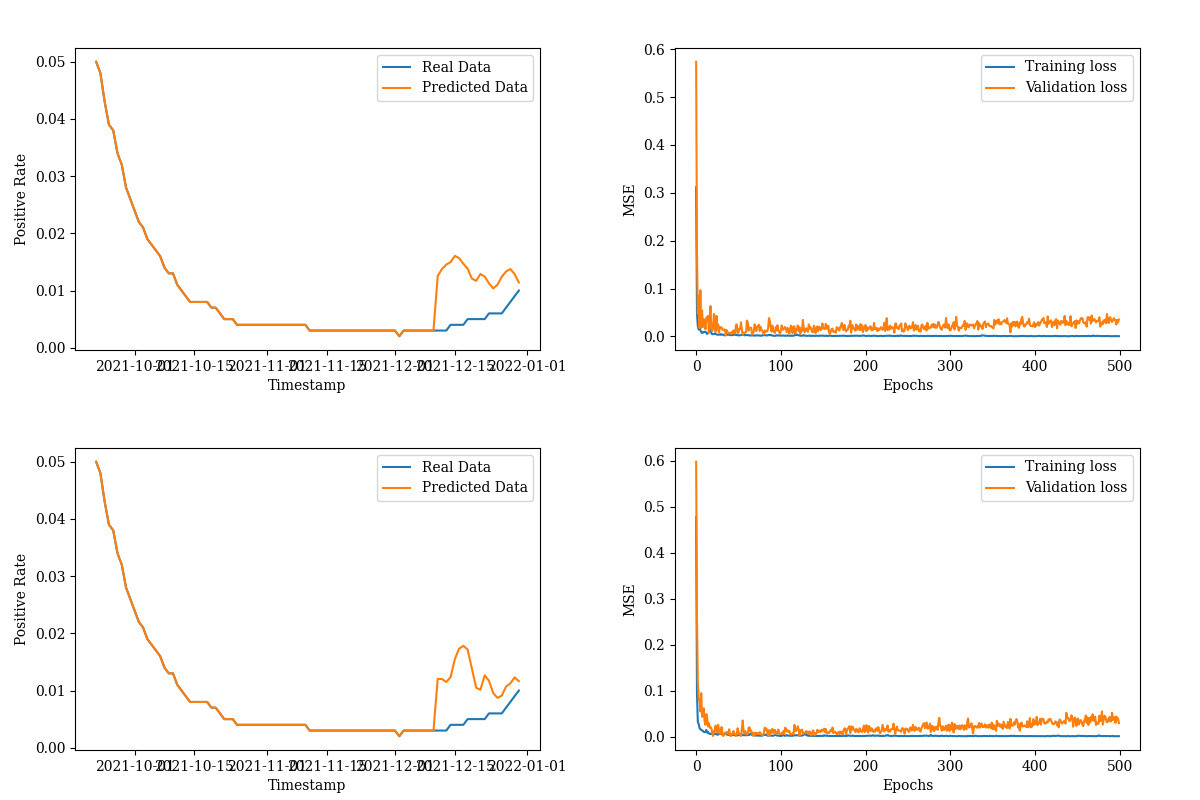
\includegraphics[width=16cm]{images/DeepLearning_Mult_20Days.jpg}
    \captionof{figure}{The line graph of produced prediction results and process of accuracy performance of multivariate prediction of 20 days. Looking at the prediction results of GRU (top-left) and LSTM (bottom-left) we could see that the model was not able to predict the objective value with high accuracy. They both have a very big spike in its prediction and has a fluctuation which is not observed in real data. The accuracy performance of both GRU (top-right) and LSTM (bottom-right) shows that despite the training loss is able to decrease its value the validation loss has a light increase trend as the epoch increases.}
    \label{fig:DL_Mult_20}
\end{figure}

\begin{figure}[!ht]
    \centering
    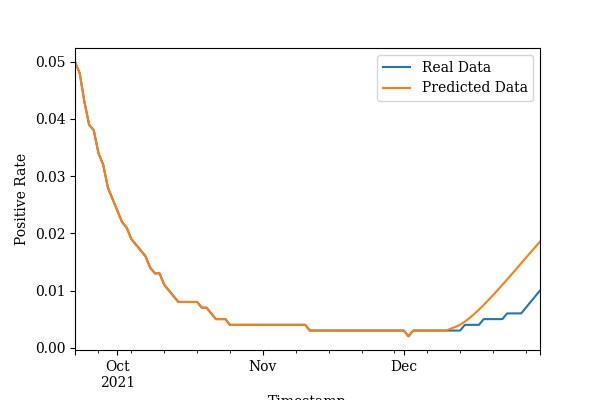
\includegraphics[width=8cm]{images/VARMA(7,2)_20Days.png}
    \captionof{figure}{The line graph of produced 20 days prediction results of VARMA(7,2) model. We could see that the prediction has a positive trend which the ARMA model was incapable of illustrate. However, we could see that the prediction line goes above the real data.}
    \label{fig:VARMA_Mult_20_line}
\end{figure}

Table \ref{tab:20Mult} shows the result of all the model performances. We could see that both neural network model was unsatisfactory of overperforming the VARMA model. However, we can see that the RMSE does not differ significantly between the models, hence an early call to say that the neural network model is ineffective in its prediction. Figures \ref{fig:DL_Mult_20}, \ref{fig:VARMA_Mult_20_line} are the line plots for the predictions. We could first see that both neural network still produce an initial spike that has persisted throughout the other neural network models. The right figures of Accuracy Performance in Figure \ref{fig:DL_Mult_20} suggest that the data itself can be properly used in the neural network and can very easily train the model with less epochs than the epochs we have set for this test. Another finding is that, the linear model for this 20 days prediction was able to account for the slight upward trend, the 40 day prediction model dismissed. This is arguably because the lag length is set at (7,2) which used the data from 7 days prior for the regression and has picked up on some elements that has shown an upward trend within the dataset. Thus, having the strongest performance out of these models. 

Overall, the univariate prediction using LSTM model performed the strongest out of all the models and the increase in features have weakened the performance for our predictions. 

\subsection{80 Days Prediction}
80 days prediction is conducted to evaluate the models' capability of capturing the sequential patterns from a smaller sample size and predict a long sequence. This is generally a difficult task since the model have to fully capture the underlying logic within data features which induces the number of observed positive rates. 

\subsubsection{Univariate Model (80 Days)}
Same as the other univariate linear models, we use ARMA(2,2) for our conventional model and compare the performance for other neural network models. 
\begin{table}[h]
\caption{Univariate Prediction Performance of Each Model (Best To Worst) - 80 Days Prediction}
    \label{tab:80Uni}
    \centering
    \begin{tabular}{ |p{3cm}||p{3cm}| }
        \hline
         Model &  RMSE\\
        \hline
        \textbf{LSTM}  & \textbf{0.001769}\\
        ARMA(2,2) & 0.008198\\
        GRU  & 0.008385\\
    \hline
    \end{tabular}
\end{table}

Table \ref{tab:80Uni} shows the evaluation for all the predictions conducted in the 3 models. We can see that the LSTM model does significantly better than the other two models. This highlights the LSTM's strength of interpreting the long term dependencies within the dataset. 

\begin{figure}[!ht]
    \centering
    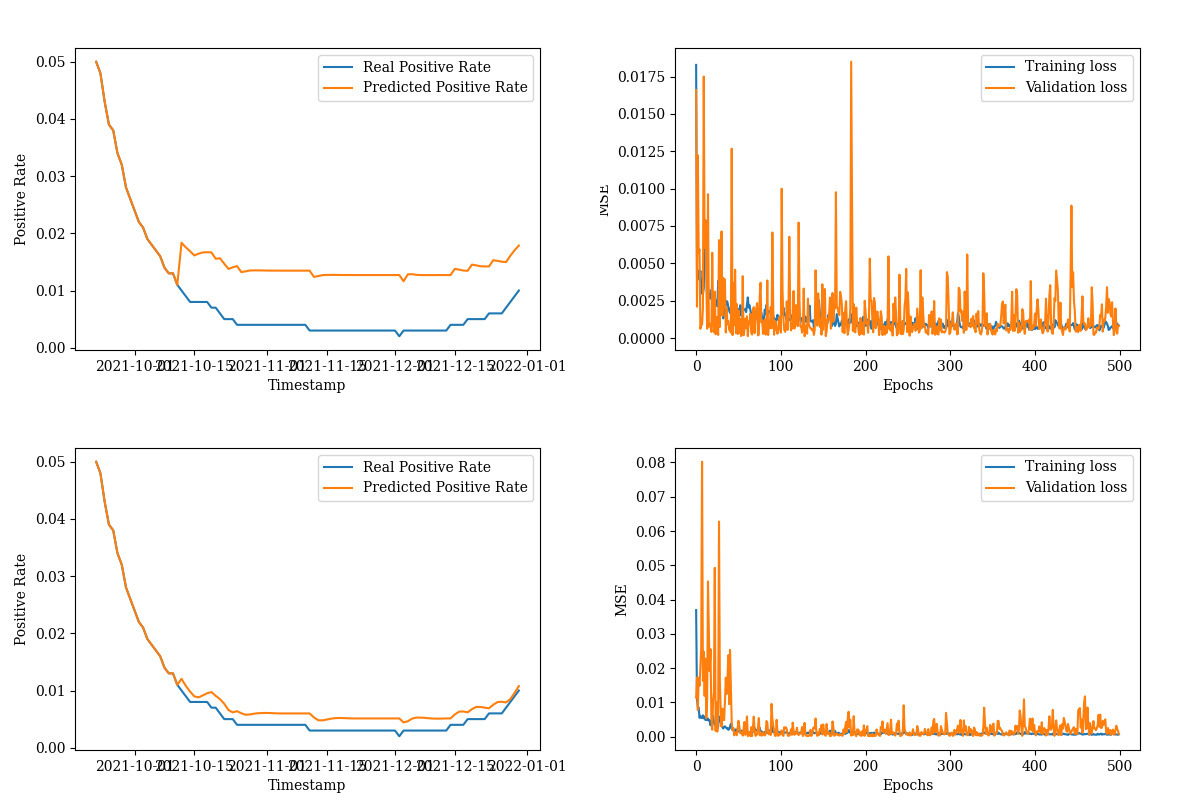
\includegraphics[width=16cm]{images/DeepLearning_Uni_80Days.jpg}
    \captionof{figure}{The line graph of produced prediction results and process of accuracy performance of the univariate prediction of 80 days. Looking at the prediction results of LSTM (bottom-left), the LSTM model was able to predict in a high accuracy with the same kind of dents. The GRU (top-left) prediction shows a spike in its first prediction, but able to illustrate the dents existing in the real data. From the accuracy performance of GRU (top-right) we could see that the training loss decreases as the epochs increase, and the validation loss is fluctuating within a small region. The accuracy performance of LSTM (bottom-right) shows that both training loss and validation loss is decreasing as the epochs increase. From both accuracy performances we can see that the neural network model is capable of being trained easily.}
    \label{fig:DL_Uni_80}
\end{figure}

\begin{figure}[!ht]
    \centering
    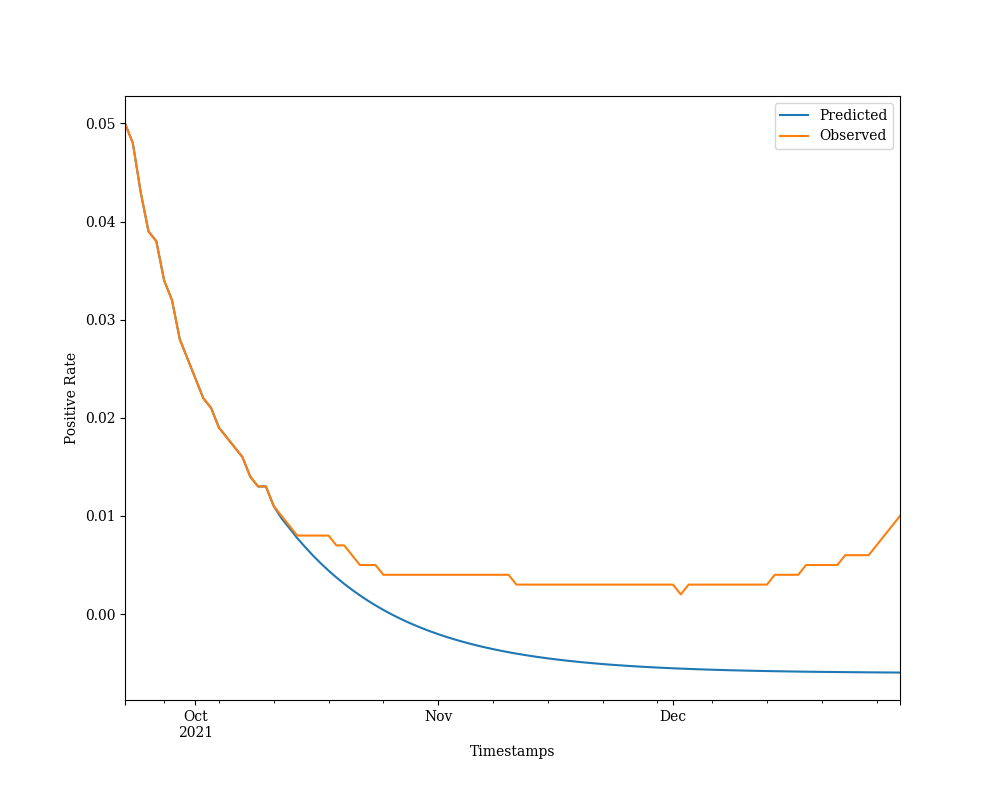
\includegraphics[width=8cm]{images/ARIMA(2,1,2)_80Days.png}
    \captionof{figure}{The line graph of produced 80 days prediction results of ARMA(2,2) model. The prediction line graph goes below the real data and has a continuing downwards trend.}
    \label{fig:ARMA_Uni_80_line}
\end{figure}

Figures \ref{fig:DL_Uni_80}, \ref{fig:ARMA_Uni_80_line} shows the prediction done by the models. Looking the Accuracy Performance figure of the bottom-right figure in Figure \ref{fig:DL_Uni_80}, the LSTM as able to predict roughly a similar curve with the same kind of dents at the corresponding time. In the context of dents, the prediction value of GRU (top-left) in Figure \ref{fig:DL_Uni_80} is also able to illustrate the dents even though the initial spike has lifted the prediction one step higher than the observed positive rates. Hence we can conclude that neural network models are capable of capturing the long term dependencies in time series data and predicting long sequence of future values.

\subsubsection{Multivariate Model (80 Days)}
We now conduct the 80 days prediction using multiple features. For the conventional method VARMA we use the lag length (2,2) with the truncated columns shown in the other VARMA models. 
\begin{table}[h]
\caption{Multivariate Prediction Performance of Each Model (Best To Worst) - 20 Days Prediction}
    \label{tab:80Mult}
    \centering
    \begin{tabular}{ |p{3cm}||p{3cm}| }
        \hline
         Model &  RMSE\\
        \hline
        \textbf{VARMA(2,2)} & \textbf{0.036689}\\
        GRU  & 0.168341\\
        LSTM  & 0.179448\\
    \hline
    \end{tabular}
\end{table}
\begin{figure}[!ht]
    \centering
    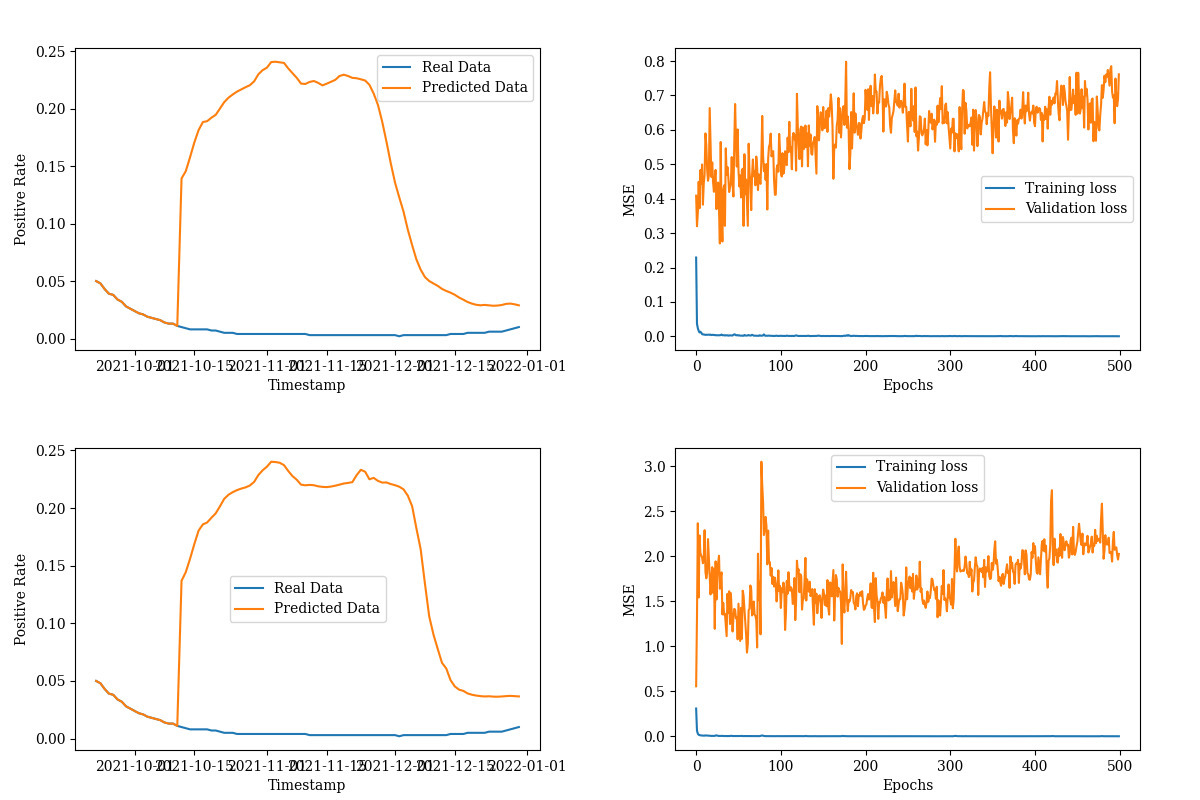
\includegraphics[width=16cm]{images/DeepLearning_Mult_80Days.jpg}
    \captionof{figure}{The line graph of produced prediction results and process of accuracy performance of multivariate prediction of 80 days. Looking at the prediction results of GRU (top-left) and LSTM (bottom-left) we could see that the model is incapable of predicting the objective values. They both have a mountain like shape in its predictions and does not look feasible. The accuracy performance of both GRU (top-right) and LSTM (bottom-right) shows that the training does not go well in both models and the validation loss is very big in both models.}
    \label{fig:DL_Mult_80}
\end{figure}

\begin{figure}[!ht]
    \centering
    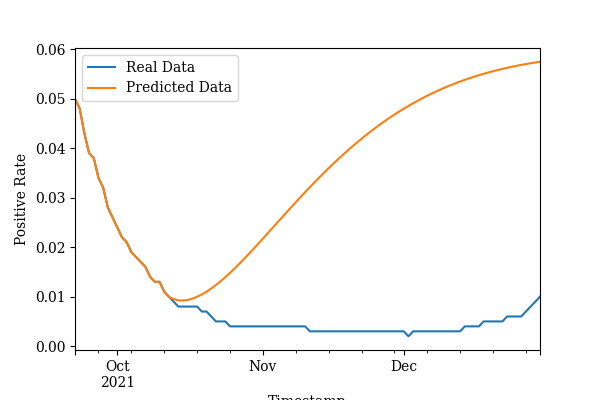
\includegraphics[width=8cm]{images/VARMA(2,2)_80Days.png}
    \captionof{figure}{The line graph of produced 80 days prediction results of VARMA(2,2) model. The prediction line graph goes above the real data and the trend of value does not reflect the actual data.}
    \label{fig:VARMA_Mult_80_line}
\end{figure}

Similarly we compile the result of RMSE for all the models and get Table \ref{tab:80Mult}. We see that the neural network models performs significantly worse compared to the VARMA(2,2) model. The RMSE of GRU and LSTM are 500\% more than the conventional model, thus we can conclude that the neural network was ineffective in its prediction using multiple variables. The prediction line figures in the left side of Figure \ref{fig:DL_Mult_80}, \ref{fig:VARMA_Mult_80_line} are the corresponding results for our predictions. We can see that the neural network models both initiates a spike and forms a mountain like shape for its prediction, which was not found in the univariate prediction models. Added to the fact that both neural network models were unable to decrease the error term in the validation data, shown in the accuracy performance in Figure \ref{fig:DL_Mult_80}, it can be concluded that the increase in features created too much noise for the neural network to be trained appropriately. 

\clearpage

\subsection{Extensive Experiments}
As shown in Sections 3.3, 3.4, 3.5 the case where the increase in features used in the neural network causing a negative affect in its prediction process has been apparent. Especially for the 80 days prediction, the Univariate model presented promising predictions as shown in the prediction line graph of LSTM model in Figure \ref{fig:DL_Uni_80} while the multivariate model was unable to show the same strong performance when it became a question of multivariate problem. For the pursuit of a better prediction result, this paper will conduct extensive experiments by adjusting the data features.

\subsubsection{Dropping Features According to the correlations}
For the multivariate predictions using neural network, we used all 9 data features to train the objective value. However, in reality there are some features that does not correlate too much with the objective value. Visualizing the correlation between the objective value and other feature values, we check the heatmap of our dataset. 

\begin{figure}[!ht]
    \centering
    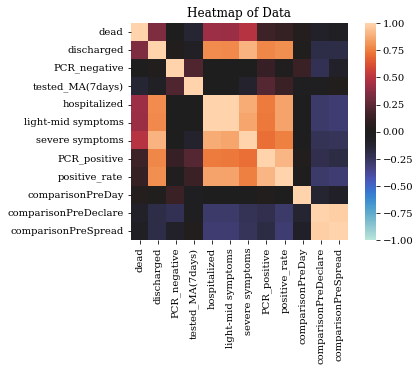
\includegraphics[width=8cm]{images/Heatmap_of_Data.png}
    \captionof{figure}{Heatmap of the Whole Dataset: The section assosiated with the objective value "Positive\_Rates" do not demonstrate strong correlation with most features}
    \label{fig:Heatmap}
\end{figure}

From Figure \ref{fig:Heatmap} we can see that there are only a few columns which shows strong correlation between the objective value. We will now define a new model which only includes the data features of Positive\_Rate, Discharged, PCR\_Positive, and ComparisonPreSpread, which are the same set of features used in the VARMA models. Naming these models LSTM\_Mod, GRU\_Mod, we compare the RMSE with the previous results. 

\begin{table}[ht]
\centering
\caption{\label{tab:Experiment1}Comparison of Multivariate Prediction Performance}
\begin{tabular}{ |p{4cm}||p{2cm}|p{2cm}|p{2cm}| }
 \hline
 Model & 40 Days & 20 Days & 80 Days \\
 \hline
VARMA & 0.021116 & 0.005607 & \textbf{0.036689} \\
LSTM & 0.030772 & 0.007889 & 0.179448\\
GRU & 0.015485 & 0.008213 & 0.168341\\
LSTM\_Mod & \textbf{0.008431} & \textbf{0.005089} & 0.175739 \\
GRU\_Mod & \textbf{0.004324} & \textbf{0.003951} & 0.170854 \\
 \hline
\end{tabular}
\end{table}
\begin{figure}[!ht]
    \centering
    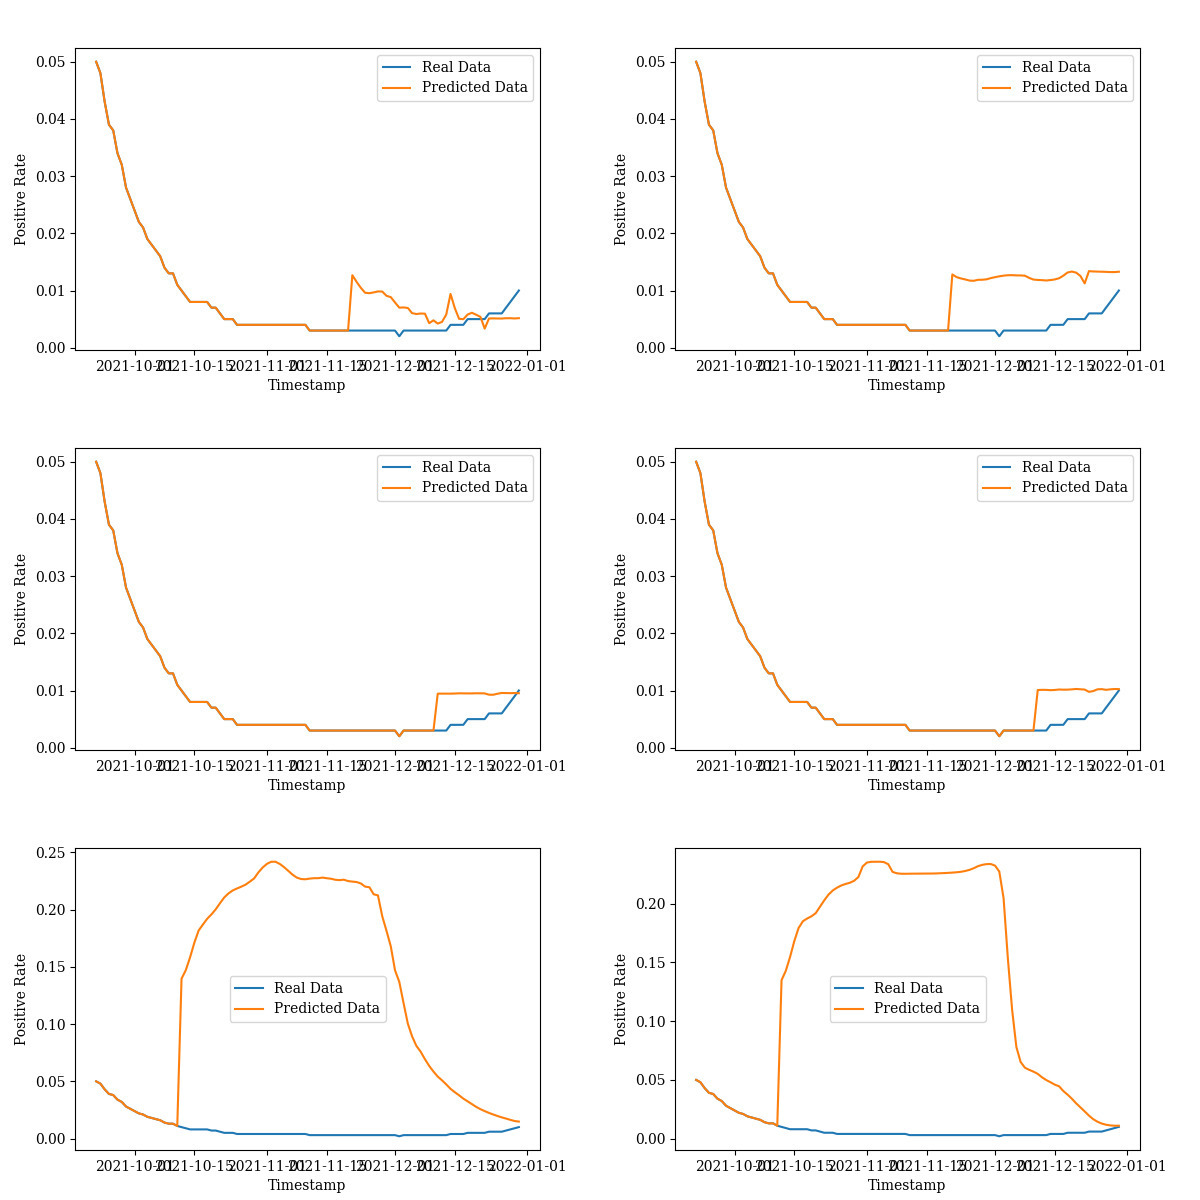
\includegraphics[width=16cm]{images/DeepLearning_Mod.jpg}
    \captionof{figure}{The line graph of prediction results produced from the modified neural network models using less features. The left side shows the prediction results from the GRU and the right side the LSTM. The top row are the 40 days prediction and both were not able to remedy the initial spike but have a downward trend which gets closer to the real data than the un-modified models. The middle row are the 20 days prediction which has an initial spike but a static value after the spike. The bottom row shows the results for the 80 days prediction and we can see that the results have a mountain shape graph but the values matches at the end for LSTM (bottom-right).}
    \label{fig:DL_Mod}
\end{figure}

As demonstrated in Table \ref{tab:Experiment1}, the modification we made, in which we decreased the number of features, have had a positive affect in terms of decreasing its RMSE for all neural network models. The less complex dataset improved their performance compared to the result without any modifications and we can conclude that extracting only the correlated features (with the assumption that all data features do not demonstrate multicollinearity) can expect improvement in our model. It still is not to the level where it outperforms the univariate prediction models but has the potential to become so. 


\subsubsection{Dropping Human Foot Traffic Data}
We have intentionally left out \textbf{ComparisonPreSpread} feature so that the model incorporates the data about how much people went outside. Since this data feature is the only data which demonstrates the human activity, which is said that it perpetuates the spread of the novel COVID-19 Virus. By comparing the prediction results with the LSTM\_Mod and GRU\_Mod model, we can determine whether the data feature of \textbg{ComparisonPreSpread} is a significant factor in our model or not. Naming the new model LSTM\_Mod\_NoHuman and GRU\_Mod\_NoHuman, this paper would compare the results with the updated model, LSTM\_Mod and GRU\_Mod made in Section 3.6.1..  
\begin{table}[ht]
\centering
\caption{\label{tab:Experiment2}Comparison of Multivariate Prediction Performance Before and After Excluding Human Foot Data}
\begin{tabular}{ |p{4cm}||p{2cm}|p{2cm}|p{2cm}| }
 \hline
 Model & 40 Days & 20 Days & 80 Days \\
 \hline
    VARMA & 0.021116 & 0.005607 & \textbf{0.036689} \\
    LSTM\_Mod & 0.008431 & \textbf{0.005089} & 0.175739 \\
    GRU\_Mod & \textbf{0.004324} & 0.003951 & 0.170854 \\
    LSTM\_Mod\_NoHuman & \textbf{0.005089} & 0.006547 & 0.177712\\
    GRU\_Mod\_NoHuman & 0.0051283 & \textbf{0.003397} & 0.169425\\
\hline
\end{tabular}
\end{table}
\begin{figure}[!ht]
    \centering
    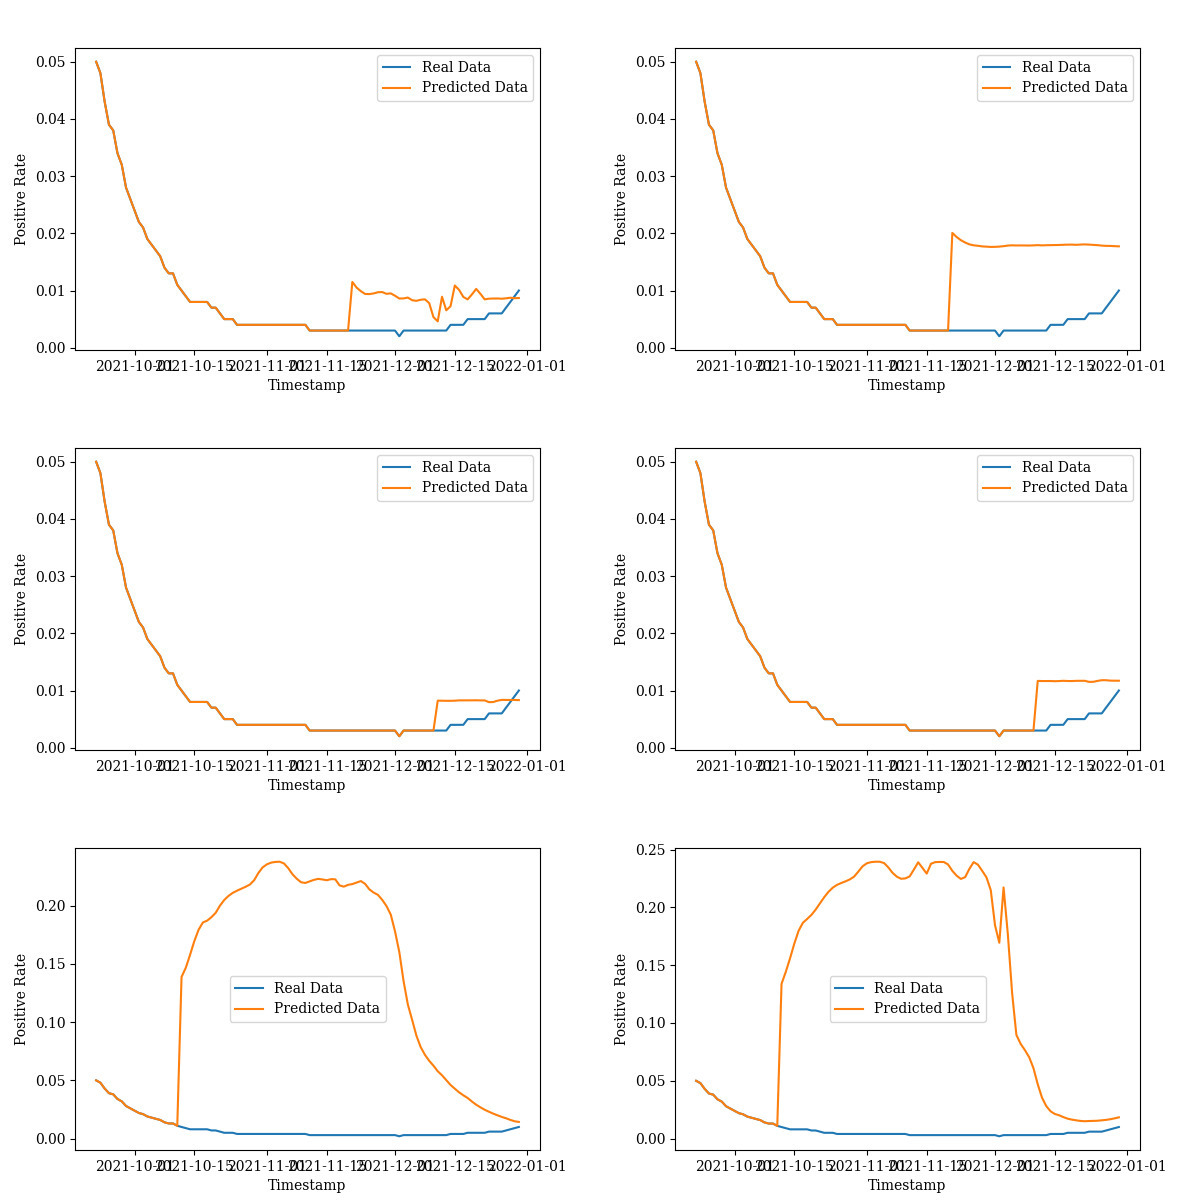
\includegraphics[width=16cm]{images/DeepLearning_NoHuman.jpg}
    \captionof{figure}{The line graph of prediction results produced from the neural network models without human activity features. The left side shows the prediction results from the GRU and the right side the LSTM. The top row are the 40 days prediction and both were not able to remedy the initial spike. The middle row are the 20 days prediction and resembles the shape of the univariate prediction curve. The bottom row shows the results for the 80 days prediction and we can see that the results still have a mountain shape graph.}
    \label{fig:DL_NoHuman}
\end{figure}

Table \ref{tab:Experiment2} shows the result for our experimentation. Looking at the LSTM model, the NoHuman version has decreased the error term in the 40 days prediction. Also for the GRU model, the 20 days prediction presents a smaller RMSE than the Mod model. Looking at the Figures in general, we could see that the \textbf{ComparisonPreSpread} feature held the value to a lower level. As it is not the case where all models performing better without human foot traffic data, and the small difference of RMSE, we cannot conclude that the data of human activity is insignificant. However, it can be seen from the mix of the features used in the model, human activity data is somewhat weak in its deterministic feature for the prediction of \textbf{Positive\_Rate}. 